\chapter{Motion}
\label{motion}

% **************************** Define Graphics Path **************************
\graphicspath{{Chapter5/Figs/}}


\section{Introduction}

Contemporary computer vision models are extremely effective at understanding individual images. So far in this thesis, we have shown deep convolutional neural network architectures which can learn powerful representations using end-to-end supervised learning. For example, in \cref{scene_understanding}, we presented models which can extract rich information at a pixel level such as semantics and geometry.
However, every algorithm so far reasons from a single image. We can only infer so much from static images. To effectively understand complex and dynamic scenes we need to reason over video.

Designing models which can learn motion and reason over temporal sequences is of critical importance for computer vision systems. Video and temporal information allows models to encode motion, reason over occlusions and improve temporal consistency and stability. Additionally, many scene understanding systems are required to inform decision making processes. Usually, these decision-making processes cannot be made in temporal isolation and, particularly in robotics, knowledge of scene dynamics is essential.

State of the art video scene understanding systems typically process individual frames independently \citep{he2017maskrcnn,zhao2017pspnet,eigen2015predicting,zhou2017unsupervised,patraucean2015spatio,valipour2017recurrent,gadde2017semantic}. Additional temporal reasoning can be performed by filtering \citep{miksik2013efficient} or with graphical models \citep{de2012line,chen2011temporally,tripathi2015semantic,hur2016joint}, however these systems are unable to be trained jointly and have significantly higher computational requirements. Many papers have proposed to add recurrent connections such as recurrent neural networks \citep{hochreiter1997long} on top of semantic segmentation encoders \citep{patraucean2015spatio,valipour2017recurrent}. However, to date, none have been able to demonstrate improvement over equivalent per-frame models at scale. In this Chapter, we observe the same result; naive sequence-to-sequence modelling from video with recurrent convolutional models harms semantic segmentation performance. We argue that this is because the recurrent units propagate their state from a static location in pixel space over time. However, in practice objects will move significantly in pixel location between consecutive frames due to camera ego-motion and scene dynamics. These models are not aware of this geometry and motion.

\begin{figure}[t]
\begin{center}
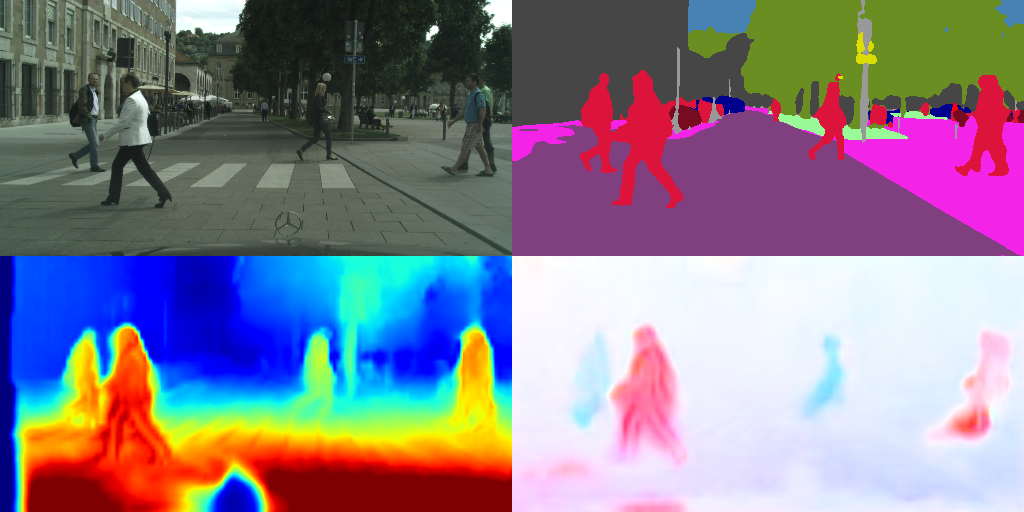
\includegraphics[width=\columnwidth,trim={7mm 12mm 7mm 0},clip]{videosegnet.png}
\end{center}
   \caption[VideoSegNet model for video scene understanding.]{\textbf{VideoSegNet model for video scene understanding.} Our model jointly learns to estimate scene motion (bottom right), depth (bottom left) and semantic segmentation (top right) over video input. Our motion-aware recurrent convolutional neural network learns semantics with supervised learning, but learns geometry and motion using unsupervised learning, without labelled training data.}
\end{figure}

In this chapter, we introduce an end-to-end deep learning architecture for video semantic segmentation which explicitly encodes motion and geometry information. Our model, which we name VideoSegNet, learns to predict optical flow and per-pixel depth estimates through unsupervised learning and semantic segmentation with supervised learning. We propose a motion-aware gated recurrent unit (motion-GRU) which is able to use motion and geometry to account for ego-motion and scene dynamics when propagating state information temporally. Since frames are usually only occasionally labelled with semantic labels, we show that learning geometry with unsupervised learning can provide a powerful dense training signal for video. We show that our model is able to perform video semantic segmentation with higher accuracy and temporal consistency than equivalent per-frame models. In summary, the novel contributions of this chapter are;
\begin{enumerate}
\item Introducing a real-time model for temporal scene understanding, VideoSegNet, which jointly learns motion, depth and semantic segmentation from video,
\item Demonstrating the importance of accounting for motion and scene geometry for video scene understanding models, and introducing temporal loss functions,
\item Showing how to train large temporal models over long video sequences at scale, improving over single-frame baselines.
\end{enumerate}

\section{Video Scene Understanding} 

\begin{figure*}[!t]
\begin{center}
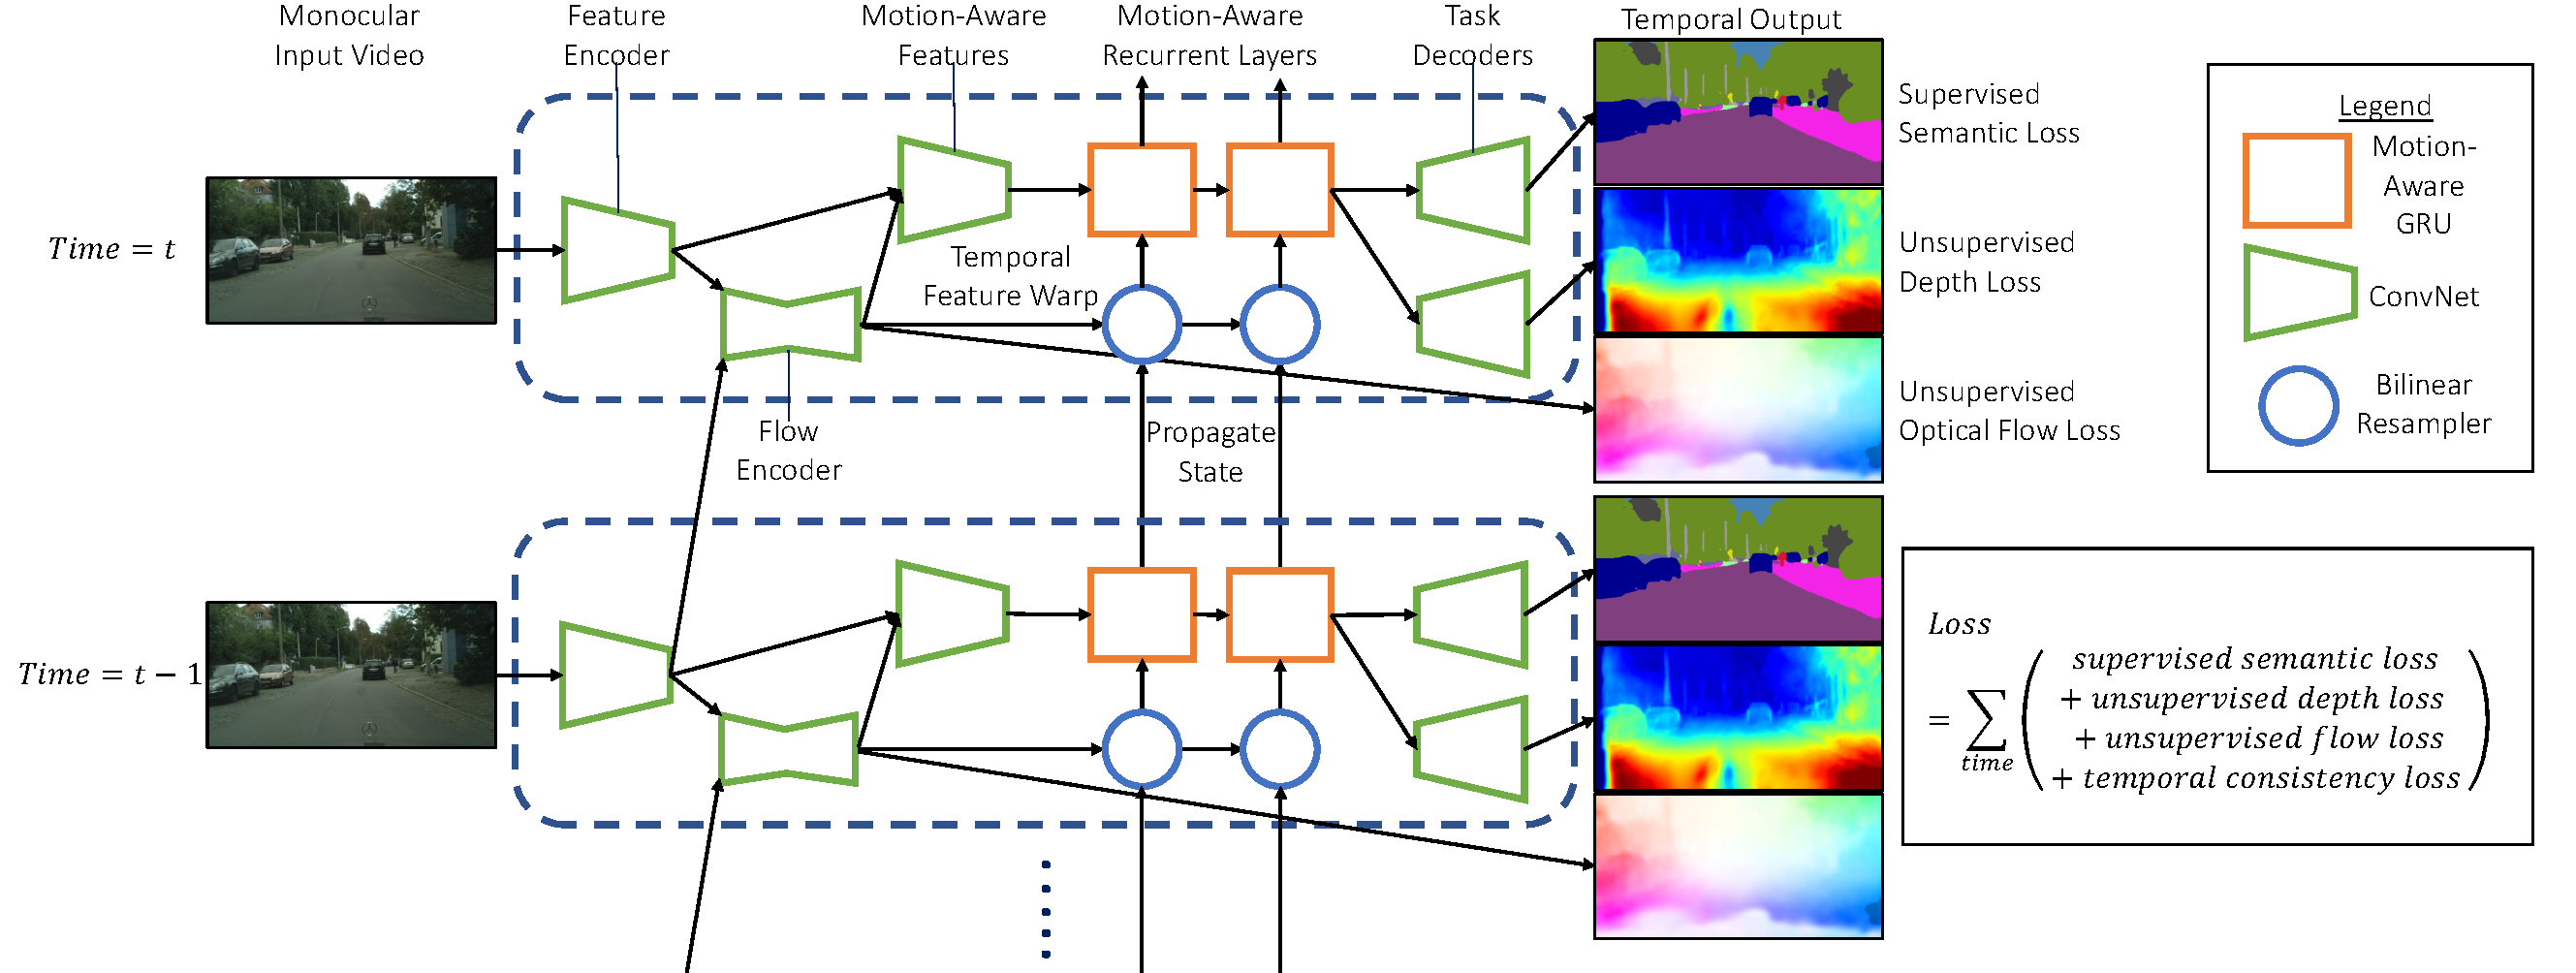
\includegraphics[width=\linewidth]{temporal_model.pdf}
\end{center}
   \caption[Overview of the VideoSegNet architecture.]{\textbf{Overview of the VideoSegNet architecture.} The model efficiently propagates information over time, outputting semantic segmentation, depth and optical flow estimate from monocular video. The model consists of three sections: firstly, learning image and motion features. Secondly, propagating information over time. Thirdly, decoding each output. In order to align features between consecutive frames we apply a warping using the predicted optical flow.}
\label{fig:arch}
\end{figure*}

Scene understanding is the task of extracting information about the objects and their contextual relationships from the observed environment. Supervised deep learning is a very effective solution to this problem from single images. In particular, many deep convolutional encoder-decoder architectures have been shown to produce accurate and real-time solutions to problems such as semantic segmentation, optical flow, depth and geometry estimation.

Semantic segmentation is the task of estimating the semantic class of each pixel in an image. State of the art models use supervised deep learning \citep{badrinarayanan2017segnet,long2015fully}, benefiting from residual architectures \citep{he2016deep,huang2017densely}. Recent work has focused on improving the receptive field of features and providing them with more context for semantic reasoning, for example using dilated convolutions \citep{YuKoltun2016} and pyramid spatial pooling \citep{zhao2017pspnet}. We have also seen semantic segmentation combined with other tasks, such as instance segmentation \citep{he2017maskrcnn} and geometry \citep{kendall2017multi} in multitask learning settings. Probabilistic modelling and Bayesian deep learning has also been used to understand model uncertainty in scene understanding algorithms \citep{kendall2017uncertainties,kendall2015bayesian}, improving safety in practical applications.

Depth and geometry models use similar architectures to semantic segmentation, but in a regression setting. Typically they estimate per-pixel metric depth or surface normals \citep{eigen2015predicting}. In \citep{UZUMIDB17} the authors learn geometry and motion using supervised learning. Deep learning models can also be trained using unsupervised learning without explicit depth labels using reprojection into stereo \citep{garg2016unsupervised} or temporal \citep{zhou2017unsupervised} frames. End-to-end deep learning can also be used to estimate depth from stereo vision \citep{kendall2017end}.

The problem of estimating motion in video is known as optical flow. Specifically, optical flow is a measurement of each pixel's 2-D motion between subsequent video frames. It captures motion due to the ego-motion of the camera (for two frames, given by the fundamental matrix \citep{hartley2000}) and motion due to scene dynamics. State-of-the-art real-time models use deep learning \citep{dosovitskiy2015flownet,flownet2} and are often trained on large synthetic datasets.

Video scene understanding, and video semantic segmentation, requires these tasks to be performed over video. Video and temporal information allows models to encode motion, reason about occlusion and improves temporal consistency and stability. Initial methods approached temporal modelling as a filtering problem \citep{miksik2013efficient}.
However, the most popular approach to date has been to construct large graphical models that connect different video pixels to achieve temporal consistency across frames \citep{de2012line,chen2011temporally,tripathi2015semantic,hur2016joint}. For example,\citep{chen2011temporally} used dynamic temporal links between the frames but optimized for a 2-D CRF with temporal energy terms.
A 3-D dense CRF across video frames is constructed in \citep{tripathi2015semantic} and optimized using mean-field approximate inference. In \citep{hur2016joint} a joint model to infer flow and semantic segmentation was proposed.

Geometry, in the form of structure from motion, has been used to aid video segmentation with random forests \citep{brostow2008segmentation} and Markov random fields \citep{tighe2013superparsing}.
More recent works look at jointly modelling 2-D semantics and 3-D reconstruction of scenes from video \citep{kundu2014joint,sengupta2013urban}.

Deep learning approaches for understanding video have been largely constrained to video level understanding tasks. For example, 3-D convolutions have been used for off-line video classification \citep{karpathy2014large} or activity recognition \citep{ji20133d}. Additionally, LSTMs have been used for video recognition and captioning \citep{donahue2015long}. However these tasks require representations at a video level, and do not need to consider scene geometry and dynamics like in this work.

Single image semantic segmentation systems have also been adapted to video segmentation. For example, \citep{gadde2017semantic} learns a representation warping module to form a two-frame video segmentation model. Clockwork convolutional networks \citep{shelhamer2016clockwork} have been proposed as a way of reducing computation for video segmentation by reusing representations from single images across time.

To date, there have been a few proposals for video segmentation models over long video sequences with deep learning \citep{patraucean2015spatio,valipour2017recurrent}. They typically append a RNN or LSTM layer after a convolutional encoder-decoder model. However, so far every model has decreased model performance, compared to single frame non-video baseline models \citep{patraucean2015spatio,valipour2017recurrent}. We believe this work is the first to demonstrate an improvement in performance using end-to-end deep learning over many-frame video sequences.

Video segmentation has also been considered in an off-line setting. This is a very different problem setting to what we consider in this Chapter, as algorithms have access to future video frames, and are not constrained to real-time inference. For example, these methods can afford to use computationally expensive spatial-temporal CRFs \citep{kundu2016feature}. In computer graphics and animation this is known as rotoscoping \citep{miksik2017roam}. Other related works of note are future video frame prediction \citep{luc2017predicting} and label propagation \citep{budvytis2010label}.

Other related work is in video object segmentation and video motion segmentation. These works are largely driven by datasets like DAVIS \citep{Perazzi2016}. This problem focuses on segmenting a single object, or moving objects \citep{tokmakov2017learning,vertens2017smsnet} in video. Unlike our work, explicit knowledge of semantics is not required. Rather, algorithms commonly use one-shot learning for masks and propagate them through video \citep{voigtlaender17BMVC}. Similar to scene understanding, the best approaches today segment single frames independently \citep{caelles2017one,khoreva2016learning}.

\section{Temporal Scene Understanding Model}

In this section we describe our model for video semantic segmentation, VideoSegNet. We describe the architecture for video scene understanding, our motion-aware recurrent neural network, our video loss function and training details.

\subsection{VideoSegNet Architecture}
\label{sec:architecture}

Consider a sequence of images, $I_0, I_1, ... , I_t$. We wish to produce a semantic segmentation output in real-time for time-step, $t$.
In order to reduce the high dimensionality of the input, we can pass the image through a deep convolutional encoder to obtain a powerful feature representation,
\begin{equation}
\mathbf{x}_t = encoder(I_t).
\end{equation}
We choose to use state-of-the-art ResNet-101 architecture for our encoder \citep{he2016deep}.

Using the feature representations from the previous and current time steps, we can then learn to regress optical flow (the motion of features between frames). We feed both these features through a network inspired by FlowNet simple \citep{dosovitskiy2015flownet}:
\begin{equation}
\mathbf{y}^{flow}_{(t-1) \to t} = flownet(\mathbf{x}_t, \mathbf{x}_{(t-1)}).
\end{equation}
This results in an estimate of optical flow for each feature from the encoder, $\mathbf{y}^{flow}_{(t-1) \to t} $. We save computation by estimating flow using features shared by the semantic encoder, rather than the raw image. This is because initial filters in flow and semantic encoders will be very similar \citep{zeiler2014visualizing}. We also improve the representation by leveraging multitask learning \citep{caruana1998multitask}.

In order to improve the feature representation for the current frame, and to incorporate motion, we concatenate the flow feature map (from the layer immediately prior to the flow regression), $\mathbf{y}'^{flow}_{(t-1) \to t}$, and the image features at the current time $\mathbf{x}_t$. We pass these features through some convolutional layers to learn a representation with motion-aware features:
\begin{equation}
\mathbf{z}_t = features(\mathbf{x}_t, \mathbf{y}'^{flow}_{(t-1) \to t})
\end{equation}
We implement $features$ as four residual layers \citep{he2016deep} with feature size $256$.

This results in a set of features, $\mathbf{z}_t$, at each time-step which encode image semantics and first order motion. Note that these features only have access to input signal from time $t$ and $t-1$. We now would like to learn long term dynamics over a sequence, to model higher-order motion and improve temporal consistency. A common approach to sequence modelling is to use a recurrent neural network (RNN). RNNs use an internal state to propagate memory over sequences. In particular, long-short-term-memory (LSTMs) units \citep{hochreiter1997long} have been shown to more effectively learn long dependencies. Gated recurrent units (GRU) \citep{cho2014learning} are a variant of LSTMs which retain the gated structure, but have a simpler internal structure making them faster to train.

Many papers have tried to place RNN or LSTM modules over features from a convolutional encoder \citep{patraucean2015spatio,valipour2017recurrent}. However, every attempt has not improved over per-frame baseline models. We make the observation that each RNN or LSTM module propagates its state forward in time for each spatial location in its feature map. However, objects in the scene rarely remain in the same location in pixel coordinates across video frames. This is due to the dynamic nature of real world environments, and ego-motion of the camera. This poses a problem for the recurrent state. This is because the state at time $t-1$, for a given pixel coordinate $(u,v)$, is unlikely to contain information about the same object which likely moved to a new pixel coordinate $(u',v')$ at the next time-step, $t$. Our hypothesis is that the propagation of misaligned features over time causes this decrease in performance with temporal models.

We propose to solve this problem by introducing a motion-aware GRU module. We know the motion of each pixel from our estimate of the optical flow, $\mathbf{y}^{flow}_{(t-1) \to t}$. Therefore we can align features over time, such that they account for motion of the object in pixel space, by warping the recurrent state and features using the estimate of optical flow. The full equations of a standard GRU are;
\begin{align}
\mathbf{g}_t &= \text{sigmoid}(W_g \cdot [\mathbf{h}_{t-1}, \mathbf{x}_t] + b_g) \\
\mathbf{r}_t &= \text{sigmoid}(W_r \cdot [\mathbf{h}_{t-1}, \mathbf{x}_t] + b_r) \\
\widetilde{h}_t &= \tanh (W \cdot [\mathbf{r}_t * \mathbf{h}_{t-1}, \mathbf{x}_t]) \\
\mathbf{h}_t &= (1-\mathbf{g}_t) * \mathbf{h}_{t-1} + \mathbf{g}_t * \mathbf{\widetilde{h}}_t,
\end{align}
with weights, $W$, and biases, $b$. To form a motion-GRU, our model is going to use its estimate of optical flow to propagate the features temporally over the video sequence, such that the features correspond in pixel space. We do this by resampling features according to the optical flow map using bilinear interpolation, inspired by spatial transformer networks (STNs) \citep{jaderberg2015spatial}.
We define this function which warps the recurrent state, $\mathbf{h}_{(t-1)}$, from time $t-1$ to time $t$, by resampling using the optical flow vectors, $\mathbf{y}^{flow}_{(t-1) \to t}$, as follows:
\begin{equation}
\mathbf{h}^{warped}_{t} = warp(\mathbf{h}_{(t-1)}, \mathbf{y}^{flow}_{(t-1) \to t}).
\end{equation}
The motion-GRU then uses $\mathbf{h}^{warped}_{t}$ rather than $\mathbf{h}_t$ as input. We backpropagate gradients smoothly by implementing this warping with bilinear interpolation \citep{jaderberg2015spatial}. We can stack multiple GRU layers in series to model long term temporal information. Note, we can also form motion-RNNs and motion-LSTMs with the same change. We choose GRUs because of their ability to gate inputs and simple implementation.

Finally, we learn separate decoders to estimate pixel-wise semantic segmentation and depth regression from the output of the motion-aware GRUs, $\mathbf{h}_t$.
\begin{align}
\mathbf{y}^{class}_t &= decoder_{class}(\mathbf{h}_t), \\
\mathbf{y}^{depth}_t &= decoder_{depth}(\mathbf{h}_t),
\end{align}
where each $decoder$ is a single $3\times 3$ convolutional layer with feature size 256 followed by a $1 \times 1$ convolutional layer regressing the required output dimensions ($1$ for depth and number of semantic classes for class).

This model can be run continuously over video in real-time to estimate per-frame optical flow, depth and semantic segmentation. This model is efficient and real-time because each image is only encoded once, and recurrent states are propagated through time. It is motion-aware from the two-frame optical flow feature input, which provides first-order motion information, and temporally aligns features. The recurrent state memory allows the model to remember higher order motion and reason over multiple views and deal with occlusion.

\subsection{Loss Function}

Our model requires us to learn three outputs: optical flow, depth regression and semantic segmentation. Optical flow and depth regression can be considered as intermediate auxiliary outputs. They assist learning semantic segmentation by making our model motion and geometry aware, improving the representation. In this section, we show how to learn semantic segmentation using supervised learning and optical flow and depth with unsupervised learning\footnote{We typically refer to this as unsupervised learning \citep{garg2016unsupervised,monodepth17,zhou2017unsupervised} due to the absence of annotated labels or the lack of the ability to evaluate the performance of the model against the data. However, this has also been referred to as \textit{self-supervision} or \textit{natural supervision} \citep{koltun2017natural} because there is a regression target and to make the distinction with unsupervised clustering.}.

Large semantic segmentation datasets are available with thousands of densely labelled images \citep{lin2014microsoft,Cordts2016Cityscapes}.
Obtaining accurate depth and flow labels is much harder. Therefore, we use an unsupervised learning regime to learn flow and depth, based on the photometric reprojection error and multi-view geometry \citep{hartley2000}. We can learn depth by learning correspondence to stereo images \citep{garg2016unsupervised} or subsequent temporal frames \citep{zhou2017unsupervised}. We can learn flow by learning correspondences between temporal frames.

More formally, to learn depth, we use the estimated disparities, $\mathbf{y}_{depth}$, from input image, $I_t$, to warp the corresponding stereo image, $I_{t,stereo}$. We train on the photometric reconstruction error to form a loss function for depth estimation:
\begin{align}
\begin{split}
\mathcal{L}_{depth,~t} = \frac{1}{N} \sum_{i,j} | I_t(i,j) - I_{t,stereo}(i,j+\mathbf{y}_{depth,t}(i,j)) |  + \lambda | \nabla \mathbf{y}_{depth,t}(i,j) |,
\end{split}
\label{eqn:depth}
\end{align}
where indices $i$ and $j$ correspond to pixel locations in the image. The loss is averaged across all temporal frames and pixels, $N$. Resampling pixel indices is performed by bilinear interpolation \citep{jaderberg2015spatial}. Minimising this loss causes the model to learn disparity, which is inversely proportional to metric depth.

The photometric reprojection error function is non-informative in homogeneous regions of the scene -- referred to as the aperture problem \citep{hartley2000}. For example, in repetitive or texture-less surfaces, multiple disparities can generate equally good losses. Only when considering wider context can we reason about these regions with sufficient information. For this reason, a prior is often applied to the loss function, typically a smoothing function, to overcome the aperture problem. Previous literature \citep{garg2016unsupervised} uses some form of the total variation (TV) loss \citep{rudin1992nonlinear}: $\nabla | Y_{depth,t} |$. Following \citep{garg2016unsupervised}, we use $\lambda = 0.01$.

For motion, we can warp the previous frame to the current frame, except now our disparity estimates have two-degrees of freedom to represent optical flow. Again, the loss is formed using the temporal, photometric reconstruction error:
\begin{align}
\begin{split}
\mathcal{L}_{flow,~t} =& \frac{1}{N} \sum_{i,j} | I_t(i,j)
- I_{(t-1)}(i+\mathbf{y}_{flow~i,t}(i,j),j+\mathbf{y}_{flow~j,t}(i,j))) |
+ \lambda | \nabla \mathbf{y}_{flow,t}(i,j) |.
\label{eqn:flow}
\end{split}
\end{align}

We learn semantic segmentation with the cross entropy loss between semantic segmentation prediction, $\mathbf{y}_{class}$, and ground truth label, $\mathbf{\hat{y}}_{class}$ for all semantic classes, $c$.
Typically, frames in video sequences are only sparsely labelled \citep{Cordts2016Cityscapes}. We therefore average the loss across only pixels and frames with ground truth labels, ignoring all others.

However, cross entropy trains each pixel independently in space and time. Additionally, we would like to encourage the network to learn a temporally consistent solution. We define a temporal consistency loss, which penalises temporal differences in segmentation prediction, after accounting for motion using optical flow:
\begin{multline}
\mathcal{L}_{consistency,~t} = \frac{1}{N} \sum_{i,j} | \mathbf{y}_{class,t}(i,j) - \mathbf{y}_{class,(t-1)}(i+\mathbf{y}_{flow~i,t}(i,j),j+\mathbf{y}_{flow~j,t}(i,j)) |,
\label{eqn:consistency}
\end{multline}
where $\mathbf{y}(i,j)$ represents the semantic logit at pixel location $i,j$. The intuition here is that, if the optical flow estimate is correct, then corresponding pixel locations should represent the same semantic class.

The total loss combines the individual losses: depth \eqn{depth}, flow \eqn{flow}, classification and consistency \eqn{consistency}. Because we are optimising multiple losses, this is a multitask learning problem \citep{caruana1998multitask}. A naive choice of overall loss would be to sum each individual loss:
\begin{equation}
\mathcal{L}_{total} = \mathcal{L}_{class} +\mathcal{L}_{flow} +\mathcal{L}_{depth} +\mathcal{L}_{consistency} .
\end{equation}

However, Kendall et al. \citep{kendall2017multi} showed that the choice of weights between the losses in deep learning models has a very strong effect on overall performance. They propose a method to learn these weights automatically by considering each task's uncertainty. We use this method to automatically weight the losses as proposed in \citep{kendall2017multi}:
\begin{equation}
\mathcal{L} = \sum_{\mathcal{L}_i \in [\mathcal{L}_{0}, \mathcal{L}_{1}, ..., \mathcal{L}_{N}]} \frac{1}{2 \sigma_i^2} \mathcal{L}_i + \log \sigma_i,
\label{eqn:multitask}
\end{equation}
where we estimate the task (homoscedastic) uncertainty of each loss, $i$, by optimising a variable, $\sigma_i$. This formulation decreases the weight for tasks which have higher variance in their residuals. This is important because we are learning outputs with many different units: semantics as probability distributions, depth as a distance and optical flow in pixels. This formulation is able to balance the losses and learn a representation which is effective for each task: flow, depth and semantic segmentation.

\begin{figure*}[p]
\clearpage
\begin{tabularx}{\textwidth}{@{}YYYYY@{}}
\hline
$\mathbf{t-10}$ & $\mathbf{t-5}$ & $\mathbf{t-3}$ & $\mathbf{t-2}$ & $\mathbf{t}$ \\
\hline
\end{tabularx}

\begin{subfigure}[t]{\linewidth}
\begin{center}
\resizebox{\linewidth}{!}{
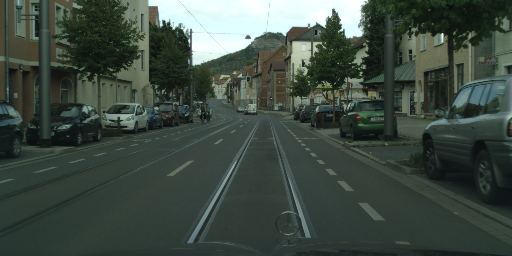
\includegraphics[width=0.15\linewidth]{seq/image_000086_000001_image.png}
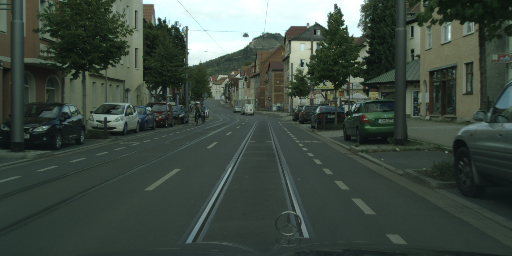
\includegraphics[width=0.15\linewidth]{seq/image_000086_000004_image.png}
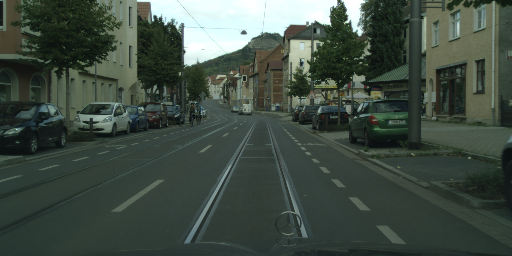
\includegraphics[width=0.15\linewidth]{seq/image_000086_000007_image.png}
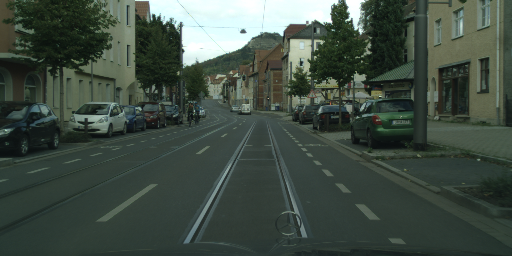
\includegraphics[width=0.15\linewidth]{seq/image_000086_000008_image.png}
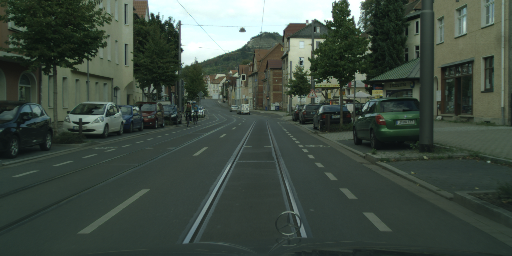
\includegraphics[width=0.15\linewidth]{seq/image_000086_000009_image.png}}
  \caption{Input video sequence}
\end{center}
\end{subfigure}

\begin{subfigure}[t]{\linewidth}
\begin{center}
\resizebox{\linewidth}{!}{
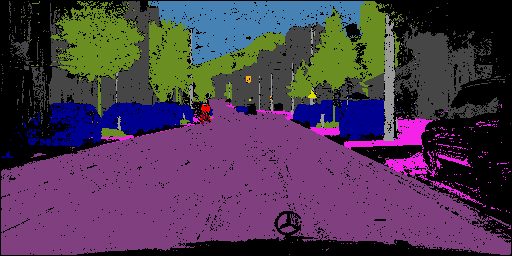
\includegraphics[width=0.15\linewidth]{seq/image_000086_000001_label.png}
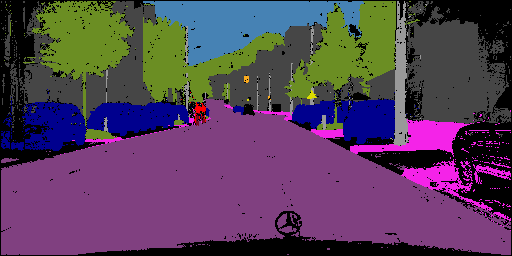
\includegraphics[width=0.15\linewidth]{seq/image_000086_000004_label.png}
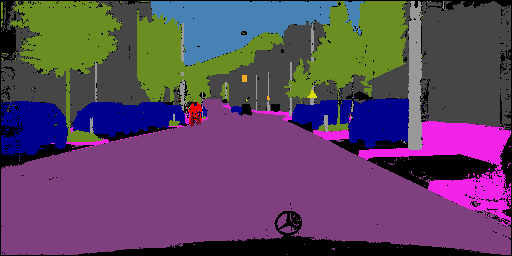
\includegraphics[width=0.15\linewidth]{seq/image_000086_000007_label.png}
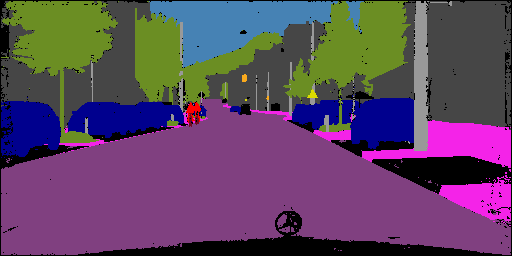
\includegraphics[width=0.15\linewidth]{seq/image_000086_000008_label.png}
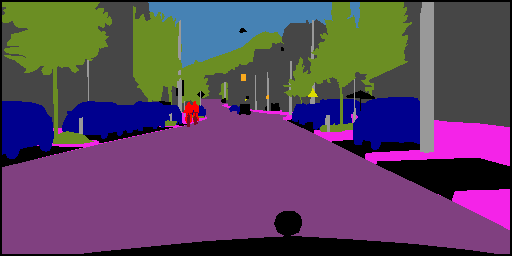
\includegraphics[width=0.15\linewidth]{seq/image_000086_000009_label.png}}
  \caption{Semantic Segmentation labels from CityScapes dataset \citep{Cordts2016Cityscapes} and propagated by \citep{budvytis2017large,budvytis2010label}}
\end{center}
\end{subfigure}

\begin{subfigure}[t]{\linewidth}
\begin{center}
\resizebox{\linewidth}{!}{
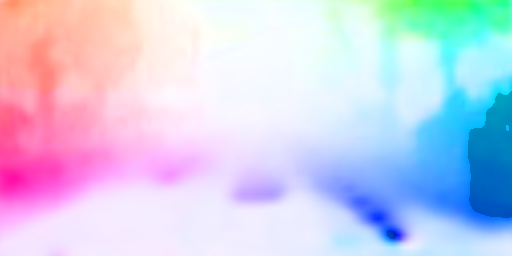
\includegraphics[width=0.15\linewidth]{seq/image_000086_000001_flow.png}
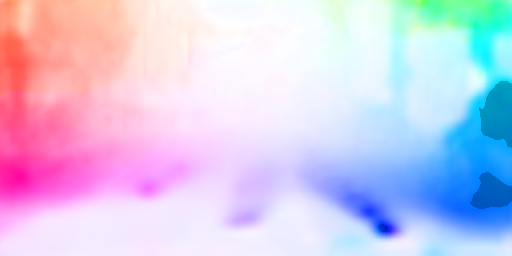
\includegraphics[width=0.15\linewidth]{seq/image_000086_000004_flow.png}
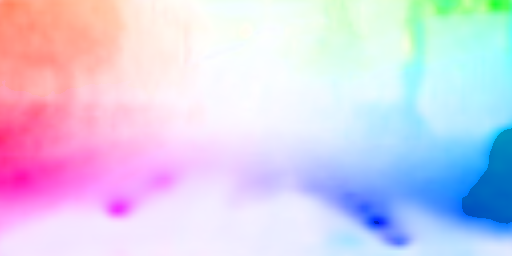
\includegraphics[width=0.15\linewidth]{seq/image_000086_000007_flow.png}
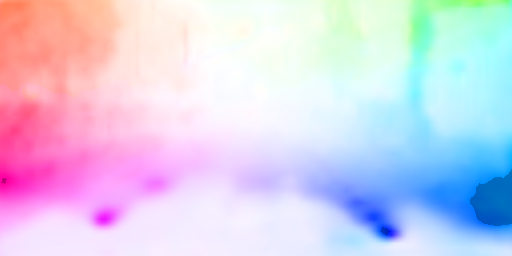
\includegraphics[width=0.15\linewidth]{seq/image_000086_000008_flow.png}
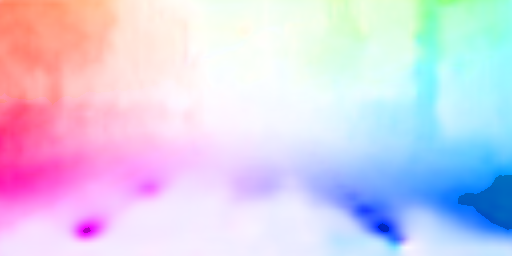
\includegraphics[width=0.15\linewidth]{seq/image_000086_000009_flow.png}}
  \caption{VideoSegNet optical flow estimation}
\end{center}
\end{subfigure}

\begin{subfigure}[t]{\linewidth}
\begin{center}
\resizebox{\linewidth}{!}{
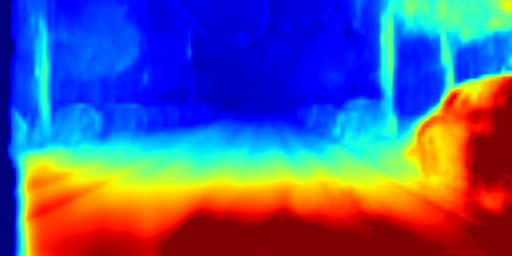
\includegraphics[width=0.15\linewidth]{seq/image_000086_000001_depth.png}
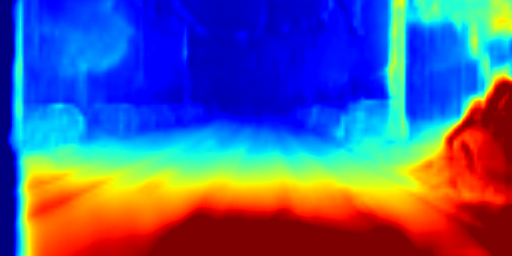
\includegraphics[width=0.15\linewidth]{seq/image_000086_000004_depth.png}
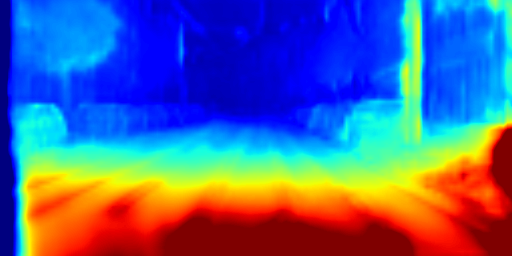
\includegraphics[width=0.15\linewidth]{seq/image_000086_000007_depth.png}
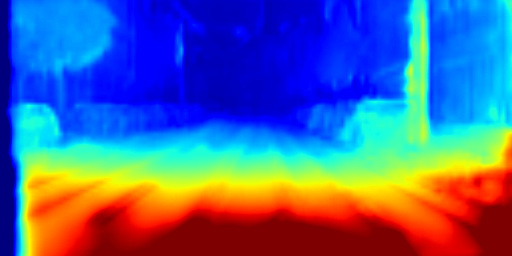
\includegraphics[width=0.15\linewidth]{seq/image_000086_000008_depth.png}
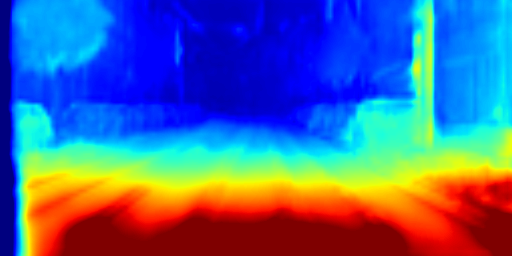
\includegraphics[width=0.15\linewidth]{seq/image_000086_000009_depth.png}}
  \caption{VideoSegNet video depth estimation.}
\end{center}
\end{subfigure}

\begin{subfigure}[t]{\linewidth}
\begin{center}
\resizebox{\linewidth}{!}{
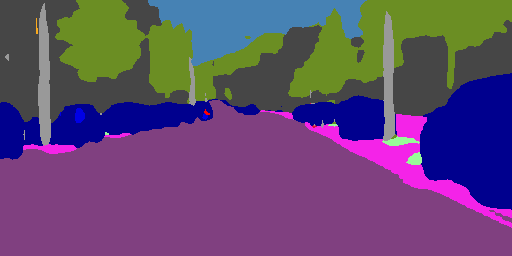
\includegraphics[width=0.15\linewidth]{seq/image_000086_000001_segmentation.png}
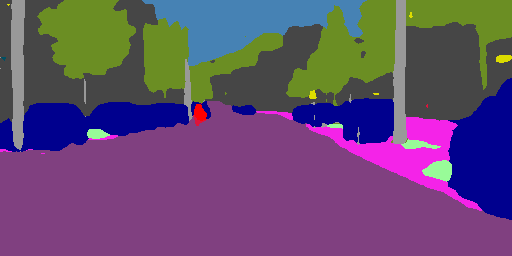
\includegraphics[width=0.15\linewidth]{seq/image_000086_000004_segmentation.png}
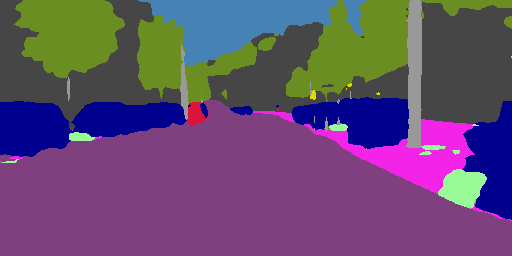
\includegraphics[width=0.15\linewidth]{seq/image_000086_000007_segmentation.png}
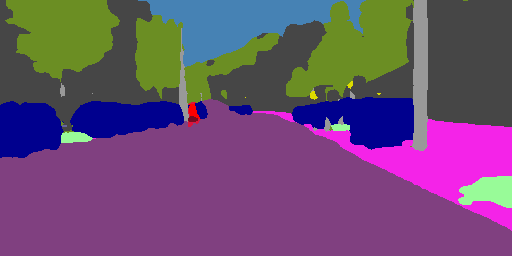
\includegraphics[width=0.15\linewidth]{seq/image_000086_000008_segmentation.png}
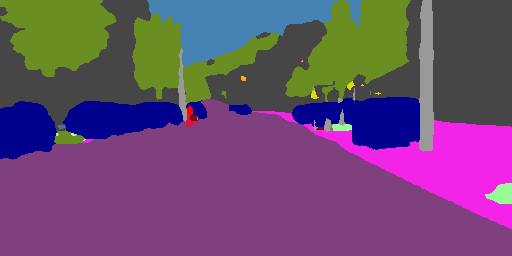
\includegraphics[width=0.15\linewidth]{seq/image_000086_000009_segmentation.png}}
  \caption{VideoSegNet video semantic segmentation.}
\end{center}
\end{subfigure}
   \caption[VideoSegNet video semantic segmentation over a 10 frame sequence.]{\textbf{VideoSegNet video semantic segmentation over a 10 frame sequence.} We observe that by learning motion and geometry and leveraging motion cues over video results in temporally consistent segmentation with less flickering between classes in the video output. We observe an increased ability to learn thin structures and difficult classes in VideoSegNet compared to the baseline. (b) also shows the propagated CityScapes labels from \citep{budvytis2017large,budvytis2010label}.}
\label{fig:results_seq}
\clearpage
\end{figure*}

\subsection{Training VideoSegNet}

We train the model over a sequence of video frames. It is important to have a number of frames so that the model can learn higher order dynamics and motion. Previous work only considers training over small sequences, often with only two frames \citep{gadde2017semantic}. Training over long sequences is very challenging, especially with large models and finite GPU memory. 

In order to fit the model on a finite GPU we train on a mini-batch with a number of video sequences with a certain time horizon, $T$. We apply the depth loss at every frame and the flow loss at every frame except the first, where it is undefined. We apply the semantic segmentation loss at every frame which contains ground truth labels (in general, not every frame will be labelled).

We find four tricks critical to achieving good performance for VideoSegNet.

\textbf{Vary training sequence length.} The first trick is to randomly vary the sequence length during training. We find that training on a fixed sequence length tends to cause the model to learn a temporally unstable representation. The recurrent state will culminate in a good representation for the fixed sequence length, but beyond this it diverges. We propose to randomly vary the sequence length, in order to train the network to learn a recurrent state which is stable over time and does not diverge.

\textbf{Train over long video sequences.} Backpropagating gradients requires significant amounts of GPU memory as feature representations from previous time-steps must be retained in memory. To overcome this, we propose to forward propagate over long (potentially infinite) video sequences, $T$, but only backpropagate over a fixed time horizon, $T'$. This allows us to discard feature activations from memory for all time-steps, except $T'$. We find this allows the model to learn representations for long term dependencies, rather than just first-order motion.

\textbf{Propagate sparse labels.} Typically, not every frame has dense pixel-wise semantic labels. While we can learn geometry and motion across all frames using unsupervised learning, this makes it hard to learn temporally consistent semantic segmentation maps. To address this, we propose to use label propagation \citep{budvytis2010label} to augment sparely labelled frames over time. This is an off-line process, taking weeks to propagate large amounts of data with graphical models \citep{budvytis2010label}. We use the dataset from \citep{budvytis2017large}, who provide propagated labels in the CityScapes dataset \citep{Cordts2016Cityscapes}, for 10 frames forward and backward from each labelled frame.

\textbf{Initialise recurrent states with identity connections.} We found that it was beneficial to initialise the recurrent connections such that they are close to identity connections \citep{he2016deep}, similar to the work of \citep{gadde2017semantic}. Ideally, we would like the initial model to be identical to a single-image segmentation model, and for the model to learn to incorporate temporal information by backpropagation. To achieve this, we set the initial bias in the GRU gates to $4.0$ so that the sigmoid function evaluates to near $1.0$. Consequently, the state will be almost entirely forgotten, and the signal almost entirely propagated from the current time-step.

While we utilise these four tricks to aid training, at test time our model can run at real-time as a Markov model, where each frame is processed only once. We do not need to retain feature activations, or historical input images, we simply propagate the latent state. At each time-step, our model is provided the current image, previous image's features (to compute optical flow) and previous motion-aware GRU state. For the first time-step, when no previous image is available, we set flow and previous state to zero.

\begin{figure*}[t]
\begin{subfigure}[t]{\linewidth}
\begin{center}
\resizebox{\linewidth}{!}{
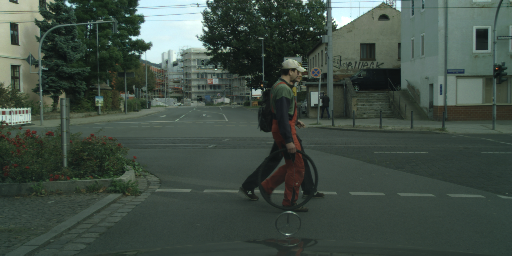
\includegraphics[width=0.15\linewidth]{image_000050_000019_image.png}
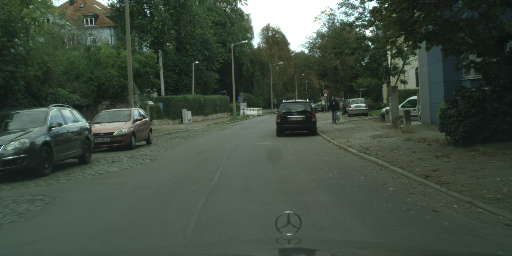
\includegraphics[width=0.15\linewidth]{image_000045_000019_image.png}
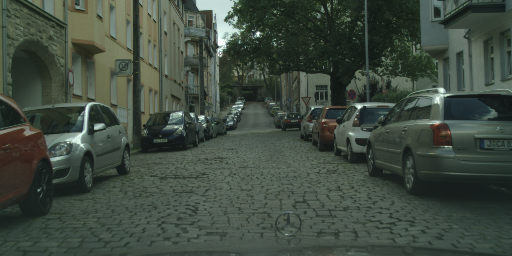
\includegraphics[width=0.15\linewidth]{image_000046_000019_image.png}
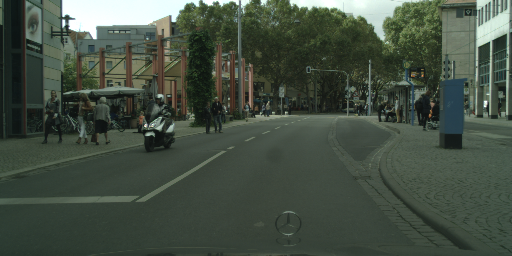
\includegraphics[width=0.15\linewidth]{image_000038_000019_image.png}
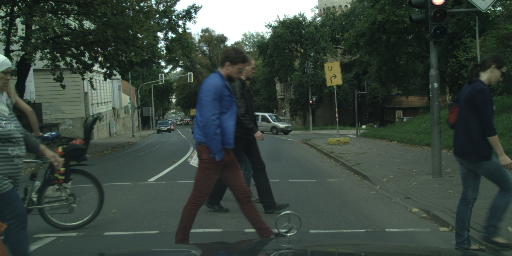
\includegraphics[width=0.15\linewidth]{image_000071_000019_image.png}}
  \caption{Input test images from video}
\end{center}
\end{subfigure}

\begin{subfigure}[t]{\linewidth}
\begin{center}
\resizebox{\linewidth}{!}{
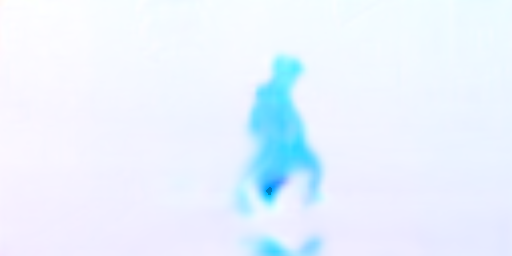
\includegraphics[width=0.15\linewidth]{image_000050_000019_flow.png}
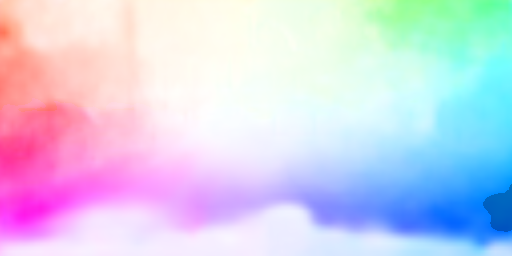
\includegraphics[width=0.15\linewidth]{image_000045_000019_flow.png}
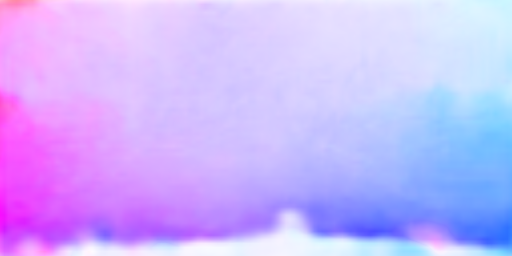
\includegraphics[width=0.15\linewidth]{image_000046_000019_flow.png}
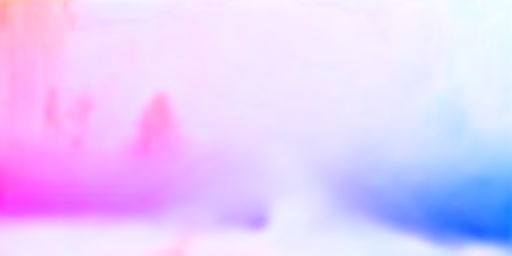
\includegraphics[width=0.15\linewidth]{image_000038_000019_flow.png}
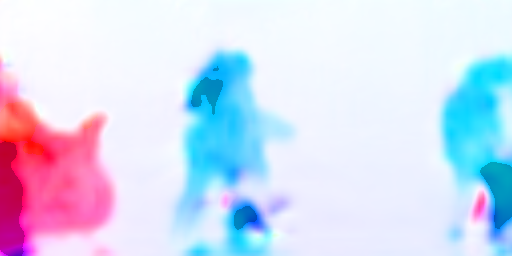
\includegraphics[width=0.15\linewidth]{image_000071_000019_flow.png}}
  \caption{VideoSegNet optical flow estimation}
\end{center}
\end{subfigure}

\begin{subfigure}[t]{\linewidth}
\begin{center}
\resizebox{\linewidth}{!}{
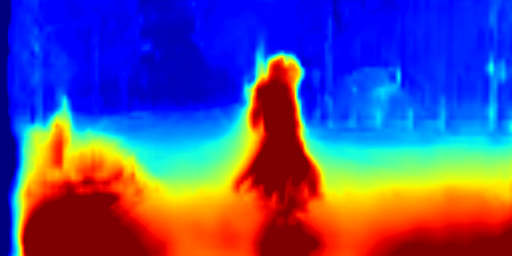
\includegraphics[width=0.15\linewidth]{image_000050_000019_depth.png}
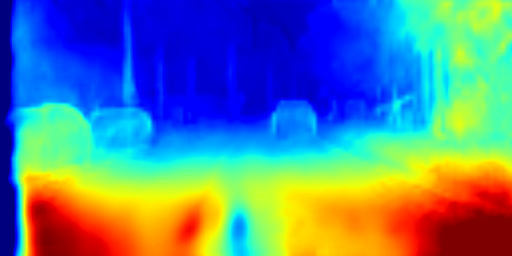
\includegraphics[width=0.15\linewidth]{image_000045_000019_depth.png}
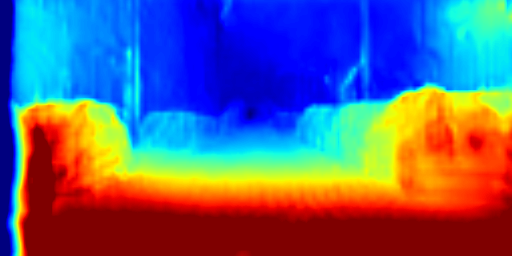
\includegraphics[width=0.15\linewidth]{image_000046_000019_depth.png}
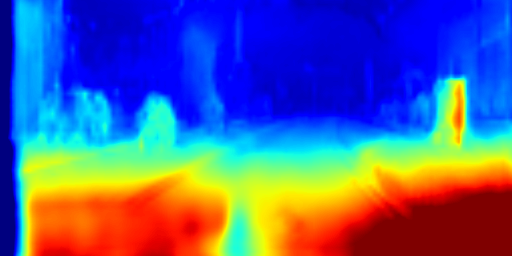
\includegraphics[width=0.15\linewidth]{image_000038_000019_depth.png}
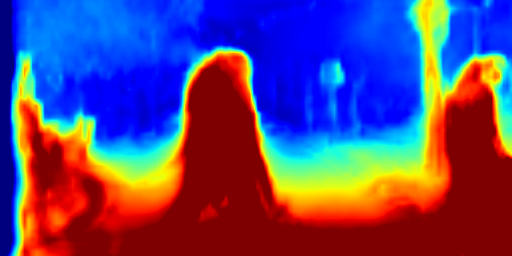
\includegraphics[width=0.15\linewidth]{image_000071_000019_depth.png}}
  \caption{VideoSegNet depth estimation}
\end{center}
\end{subfigure}

\begin{subfigure}[t]{\linewidth}
\begin{center}
\resizebox{\linewidth}{!}{
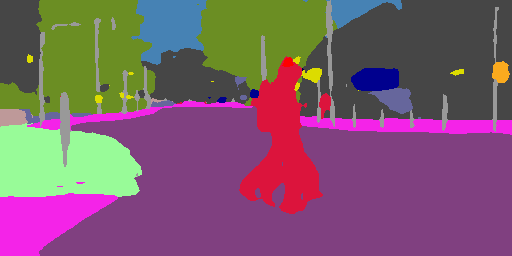
\includegraphics[width=0.15\linewidth]{image_000050_000019_segmentation.png}
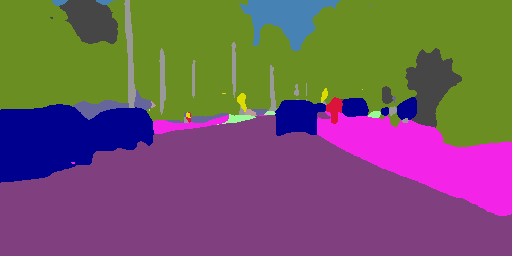
\includegraphics[width=0.15\linewidth]{image_000045_000019_segmentation.png}
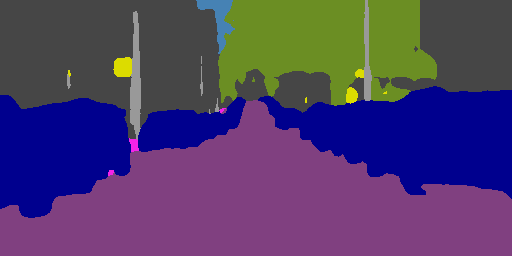
\includegraphics[width=0.15\linewidth]{image_000046_000019_segmentation.png}
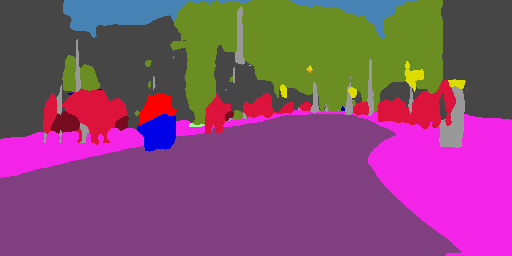
\includegraphics[width=0.15\linewidth]{image_000038_000019_segmentation.png}
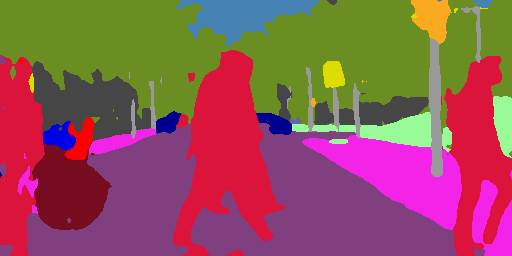
\includegraphics[width=0.15\linewidth]{image_000071_000019_segmentation.png}}
  \caption{VideoSegNet semantic segmentation}
\end{center}
\end{subfigure}
   \caption[VideoSegNet qualitative results.]{\textbf{VideoSegNet qualitative results} for video semantic segmentation, optical flow and depth estimation.}
\label{fig:results}
\end{figure*}

\section{Experiments}

In this section we perform a number of experiments to evaluate the importance of compensating for motion in our architecture in addition to other design decisions. We also benchmark our model against other approaches. 

\textbf{Dataset.} We use the CityScapes dataset for all experiments \citep{Cordts2016Cityscapes} which is a road scene understanding dataset. The CityScapes dataset was taken from a vehicle in various locations around Germany. It provides $5000$ stereo images with $1024 \times 2048$ resolution (of which $3,500$ are for training) with dense semantic segmentation labels. It also provides $20$ preceding and $10$ future frames around each labelled frame. Therefore, one time-step in this sequence will have semantic labels, and we can apply the other unsupervised losses at every time-step. In some experiments, we also make use of the propagated CityScapes dataset \citep{budvytis2017large}. 

In order to train VideoSegNet in GPU memory, we sub-sample CityScapes images to $256\times 512$ resolution for training and testing. Training and benchmarking on the full $1024\times2048$ CityScapes benchmark was not possible, due to the onerous memory demands of training over large resolution video. We leave this comparison to future work.

\textbf{Metrics.} We evaluate semantic segmentation performance with three metrics. First, mean intersection over union (IoU) measures the pixel wise semantic performance. It penalises false negatives and false positives. We also evaluate the boundary intersection over union (bIoU) \citep{badrinarayanan2017segnet}, which provides more granularity by only testing across pixels near class boundaries. This more aggressively tests accuracy and performance around thin and challenging objects.

We also evaluate the temporal consistency (TC) of the labels to evaluate if our video model produces more consistent and coherent results. To do this we compute the optical flow tracks over frames preceding the labelled image, using the predicted optical flow. We define temporal consistency as the percentage of pixels along an optical flow track which have the same class prediction.

Unfortunately, we cannot easily evaluate optical flow and depth performance, as these quantities are learned with unsupervised learning without labels. However, the CityScapes dataset does provide depth labels from stereo \citep{Cordts2016Cityscapes} which we use to compute depth error metrics.

\textbf{Optimisation.} For all experiments, we use a batch size of four, placing each video sequence on a separate GPU, using a machine with four NVIDIA Titan X GPUs. We train with stochastic gradient descent, with $0.9$ momentum and a base learning rate of 0.01. We decay this learning rate using a polynomial schedule \citep{chen14semantic}. We use ResNet-101 weights pretrained on ImageNet \citep{he2016deep}, and apply a $0.1$ learning rate multiplier to these weights during training.

\subsection{Ablation Studies}
In this section, we quantify the effect of a number of design choices in VideoSegNet and justify our architecture against various baselines. To reduce computational burden, we perform experiments on the CityScapes dataset with images at quarter resolution of 512x256 pixels. We use a batch size of four with a training time horizon of four, unless otherwise specified. We train over $150k$ iterations.

\textbf{Importance of temporal models.} In \sct{architecture} we presented the hypothesis that temporal convolutional models using recurrent units degraded performance compared to equivalent per-frame models, however our motion-aware recurrent model would effectively capture motion and improve performance. In \tbl{motion} we compare the different models to answer this question.
Appending a recurrent layer to the per-frame baseline, as was proposed by \citep{patraucean2015spatio,valipour2017recurrent}, reduces performance.
Adding in our motion-aware GRU and the temporal consistency loss significantly improves performance over both the GRU model and the per-frame baseline. This demonstrates that accounting for motion in video models is extremely beneficial.
In addition, our temporal consistency loss further improves performance by explicitly enforcing temporal consistency during training.

\begin{table}[h]
\begin{center}
	\begin{tabular}{l|c|c|c}
    \hline
    Model & IoU & bIoU & TC \\
    \hline\hline
    baseline (no motion) & 63.9\% & 43.1\% & 72.8\% \\
    1 GRU & 63.5\% & 43.1\% & 75.8\% \\
    1 motion-GRU & 65.6\% & 45.3\% & 81.4\% \\
    2 motion-GRU & 65.8\% & \textbf{45.5\%} & 82.2\% \\
    2 motion-GRU + consistency & \textbf{65.9\%} & 45.1\% & \textbf{88.2\%} \\
    \hline
	\end{tabular}
\end{center}
\caption[Importance of modelling motion.]{\textbf{Importance of modelling motion.} We compare our motion-GRU to baseline models and quantify the improvement due to modelling motion with segmentation intersection over union (IoU), boundary-IoU (bIoU) and temporal consistency (TC). These results show that naively adding recurrent units to a segmentation model degrades performance. Modelling motion with our proposed motion-aware recurrent architecture improves performance. Our temporal consistency loss improves results further.}
\label{tbl:motion}
\end{table}

\textbf{Importance of geometry.}
In \tbl{multitask} we observe a large quantitative improvement in results by modelling geometry. Learning with motion and depth features significantly improves performance. We find that introducing the multitask loss \citep{kendall2017multi} helps to correctly weight the losses, improving results further.

\begin{table}[h]
\begin{center}
	\begin{tabular}{l|c|c|c}
    \hline
    Tasks & IoU & bIoU & TC \\
    \hline\hline
    semantics & 63.3\% & 42.8\% & 71.0\% \\
    semantics+depth & 63.9\% & 43.1\% & 72.8\% \\
    semantics+motion & 65.8\% & 45.5\% & 82.2\% \\
    semantics+motion+depth & 66.1\% & 46.3\% & 82.6\% \\
    \begin{tabular}{@{}c@{}}semantics+motion+depth \\ +multitask loss \citep{kendall2017multi}\end{tabular} & \textbf{66.4\%} & \textbf{46.5\%} & \textbf{82.9\%} \\
    \hline
	\end{tabular}
\end{center}
\caption[Benefit of multitask learning.]{\textbf{Benefit of multitask learning.} These experiments illustrate the improvement our approach receives from multitask learning. Learning representations of motion and geometry significantly improves performance of semantic segmentation.}
\label{tbl:multitask}
\end{table}

\textbf{Sequence training.}
Using the full model, we also compare the effect of training over different length time-steps in \tbl{timesteps}. We observe an improvement with training over longer time sequences, including with a `warmup' when the sequence is too long to backpropagate in memory. Training with propagated labels further improves the model.

\begin{table}[h]
\begin{center}
	\begin{tabular}{l|c|c|c|c|c}
		\hline
		Timesteps & \begin{tabular}{@{}c@{}}Label\\prop\end{tabular} & IoU & bIoU & TC & Depth \\
		\hline\hline
        1 & & 63.9\% & 43.1\% & 72.8\% & 14.0 \\
		2 & & 64.6\% & 44.2\% & 81.0\% & 9.2 \\
		4 & & 65.9\% & 45.1\% & 88.2\% & 8.7 \\
		4 & \checkmark & 67.2\% & 49.2\% & 93.1\% & 8.9 \\
		4 + 4 warmup & & 66.1\% & 45.4\% & 88.3\% & 8.5 \\
        4 + 8 warmup & & 66.2\% & 45.4\% & 88.4\% & 8.5 \\
        4 + 8 warmup & \checkmark  & \textbf{68.3\%} & \textbf{50.7\%} & \textbf{95.0\%} & \textbf{8.6} \\
		\hline
	\end{tabular}
\end{center}
\caption[Method and sequence used for training video models.]{\textbf{Method and sequence used for training video models} has a massive impact on model performance. We make three observations. First, training over longer sequences improves performance. Second, propagated labels \citep{budvytis2010label} improve the model. Finally, depth estimate improves significantly with motion information. We quantify performance with intersection over union (IoU), boundary-IoU (bIoU) \citep{badrinarayanan2017segnet} and temporal consistency (TC). Depth results are given as mean absolute disparity error.}
\label{tbl:timesteps}
\end{table}

% \subsection{CityScapes Benchmark}

% We benchmark our model on the CityScapes leaderboard \citep{Cordts2016Cityscapes} to compare to other semantic segmentation methods. We train our model on $512\times 512$ resolution crops with batch size 4. We train over 4 timesteps, using warm-up of 8 timesteps. We use stochastic gradient descent with learning rate 0.01, with polynomial decay over 100,000 iterations. We use momentum of 0.9.

% \begin{table}[h]
% 	\begin{center}
% 		\begin{tabular}{l|c|c}
%         \hline
%         Method & Video & IoU \\
%         \hline\hline
%         Video Net (this work) & \checkmark &\\
%         NetWarp & \checkmark &\\
%         PSP Net  &&\\
%         Adelaide &&\\
%         Dilation Net \citep{YuKoltun2016} &&\\
%         FCN \citep{long2015fully} &&\\
%         SegNet \citep{badrinarayanan2017segnet} &&\\
%         \hline
% 		\end{tabular}
% 	\end{center}
% 	\caption{Results on the CityScapes leaderboard using the held out test set.}
% 	\label{tbl:cityscapes}
% \end{table}

% In Figure ?? we show qualitative output of our model. VideoSegNet is able to produce temporally consistent frames. Despite the unsupervised training losses, VideoSegNet produces sharp and accurate optical flow and depth maps.

\textbf{Efficiency.}
On a single NVIDIA Titan Xp GPU, VideoSegNet takes $160$ milliseconds for $512 \times 246$ images. We are confident that this framework could be made even faster for real-time applications, as it adds a relatively small computational cost over single-frame semantic segmentation models. Unlike NetWarp \citep{gadde2017semantic}, we do not need to re-encode the previous image to learn motion. Rather, our model can propagate state as a Markov model.

\section{Conclusions}

In this chapter, we investigated the problem of video scene understanding. We briefly summarise the main conclusions within the three main themes of this dissertation.

\textbf{End-to-end deep learning.}
In this chapter, we have demonstrated an end-to-end deep learning model to learn semantic segmentation, optical flow and scene depth from video sequences in real-time. We show how to design recurrent units which can compensate for ego-motion and align features over time. Through a number of experiments, we present insights for training temporal models to form temporally consistent representations from long video sequences. We find that end-to-end learning over long video sequences outperforms models trained on individual frames.

\textbf{Geometry.}
We show that explicitly modelling geometry, in the form of depth and motion, is critical to obtain accurate feature representations over video sequences. We demonstrate how to use geometry to align features over time, improving segmentation performance. This allows us to improve on the per-frame segmentation model by leveraging motion features. Jointly representing depth, in addition to semantics, further improves model performance.

We find that in order to train over long video sequences, it is important to provide a training signal for each frame. Labelling the semantics of each frame is too expensive. Therefore we demonstrate that learning motion and depth with unsupervised learning is an effective method to provide a training signal for each image in a long video sequence.

\textbf{Uncertainty.}
While the probabilistic techniques from the previous chapters can be applied to this model, this chapter does not explicitly explore the application of uncertainty to the problem of video scene understanding. However, we utilise uncertainty for multitask learning using the technique from \cref{sec:multitask} to simultaneously learn depth, motion and semantics.

